%\documentclass{book}\usepackage{sjtfonts}\usepackage{includegraphics}\usepackage{alltt}\usepackage{latexsym}
%\usepackage{array}
%\begin{document}\input{defs0}%		miradefs.tex 		    June 1994

% opening and closing a quoted Miranda section

\newcommand{\mira}{\noindent\hrulefill\nopagebreak\so}
\newcommand{\arim}{\nopagebreak\st\hrulefill\\}

% backslash in the Miranda environment
% Only feasible approach is to use \verb+\+
% in line!

%\newcommand{\bs}{$\mi\backslash\!\!$}
%\newcommand{\lbs}{\mbox{\verb+\+}}

% ignoring part of the input

\newcommand{\ignore}[1]{}

% a blank line in a Miranda section

\newcommand{\bl}{\mbox{\ }}

% Signalling a diffculty.

\definecolor{light-gray}{gray}{0.95}

\newcommand{\beware}[2]
 {\medskip\noindent\colorbox{light-gray}{\parbox{\textwidth}
 {\mbox{\large\textbf{#1}} \medskip\noindent\\ #2}\medskip\noindent}}

% Subscripting in Miranda text
\newcommand{\subscr}[2]{\mbox{${\mbox{\texttt{#1}}}_{\mbox{\texttt{#2}}}$}}

%\newcommand{\subscr}[2]{\mbox{${\mbox{\mi #1}}_{\mbox{\smtt #2}}$}}
\newcommand{\aone}{\subscr{a}{1}}
\newcommand{\atwo}{\subscr{a}{2}}
\newcommand{\ak}{\subscr{a}{k}}

\newcommand{\aoneone}{\subscr{a}{1,1}}

\newcommand{\eone}{\subscr{e}{1}}
\newcommand{\etwo}{\subscr{e}{2}}
\newcommand{\ei}{\subscr{e}{i}}
\newcommand{\er}{\subscr{e}{r}}

\newcommand{\fone}{\subscr{f}{1}}
\newcommand{\fl}{\subscr{f}{l}}

\newcommand{\gone}{\subscr{g}{1}}
\newcommand{\gtwo}{\subscr{g}{2}}
\newcommand{\gi}{\subscr{g}{i}}
\newcommand{\gr}{\subscr{g}{r}}

\newcommand{\hone}{\subscr{h}{1}}
\newcommand{\hl}{\subscr{h}{l}}

\newcommand{\pone}{\subscr{p}{1}}
\newcommand{\ptwo}{\subscr{p}{2}}
\newcommand{\pk}{\subscr{p}{k}}

\newcommand{\qone}{\subscr{q}{1}}
\newcommand{\qtwo}{\subscr{q}{2}}
\newcommand{\qk}{\subscr{q}{k}}

\newcommand{\rone}{\subscr{r}{1}}
\newcommand{\rtwo}{\subscr{r}{2}}

\newcommand{\tone}{\subscr{t}{1}}
\newcommand{\ttwo}{\subscr{t}{2}}
\newcommand{\tn}{\subscr{t}{n}}

\newcommand{\vone}{\subscr{v}{1}}
\newcommand{\vtwo}{\subscr{v}{2}}
\newcommand{\vn}{\subscr{v}{n}}

% for regular expressions

\newcommand{\stone}{\subscr{st}{1}}
\newcommand{\sttwo}{\subscr{st}{2}}
\newcommand{\stn}{\subscr{st}{n}}
\newcommand{\rthree}{\subscr{r}{3}}

\newcommand{\eps}{$\varepsilon$}
\newcommand{\trans}[1]{\stackrel{\mbox{\tt #1}}{\longrightarrow}}



% superscript in Miranda text

\newcommand{\superscr}[2]{\mbox{${\mbox{\mi #1}}^{\mbox{\smtt #2}}$}}

% Not equals in Miranda text

\newcommand{\noteq}{\makebox[0pt][l]{=}/}
\newcommand{\overslash}{\makebox[0pt][l]{/}}

% Definitions in complexity chapter

\newfont{\oldSym}{cmsy10}
\newcommand{\Th}{\boldmath$\oldSym\Theta$}
\newcommand{\pow}[1]{\^{}#1}
\newcommand{\leqq}{$\leq$}
\newcommand{\geqq}{$\geq$}
\newcommand{\lll}{$\ll$}
\newcommand{\eqq}{$\equiv$}
\newcommand{\ltwo}{\subscr{log}{2}}

% Indexing

\newcommand{\minx}[1]{\index{#1@{\ttfamily{}#1}}}
\setcounter{chapter}{17}\setcounter{page}{363}

\chapter{Abstraction: functors, monads and folding}
\chapstart
\label{actions}
\index{actions|(}

This chapter introduces some of the key abstractions of the Haskell type / class system, central to which is the notion of a \textbf{monad}. A monad provides the infrastructure for sequencing and naming used in the \texttt{do} notation, and we will show instances of the \texttt{Monad} class for lists, the \texttt{Maybe} type, a parsing monad and more. Before we do that we also introduce the \texttt{Functor} and \texttt{Applicative} classes on which \texttt{Monad} is built.

The chapter then looks again at I/O in Haskell, particularly focussing on the \texttt{do} notation which we can use to write all sorts of different programs, including ones that manipulate state, that non-deterministically return more than one result, or indeed none, as well as programs that may fail, or raise exceptions. 

As well as looking at these definitions, we will program a number of examples, showing how a monadic style, using \texttt{do}, makes programs more readable and flexible.
Each instance of a monad gives a `little language' for writing programs, and we'll come back to look at this in detail in the next chapter.

\section{Abstraction}
\label{abstraction}
\index{abstraction}

This section talks about abstraction and the way it is reflected in some of the standard type classes of Haskell. We talked earlier about abstraction as a question of spotting a pattern — maybe in some data, or maybe in a computation — and representing it directly as an object, as something in the language: an artifact in the language. We talked about spotting the pattern of mapping along a list: taking a function and applying that function \texttt{f} to every element of the list. 
\begin{alltt}
map :: (a -> b) -> [a] -> [b]
\end{alltt}
In this definition we're saying: apply \texttt{f} to every element of the list. But why just lists? We could think, why not apply f to every element in the data structure? In other words, we can think of mapping across data structures other than lists.

We also saw the idea of folding: taking a function which combines all the elements of a list.
\begin{alltt}
foldr :: (a -> b -> b) -> b -> [a] -> b

foldr g s []     = s
foldr g s (x:xs) = g x (foldr g s xs)   
\end{alltt}
We saw that this pattern embodied primitive recursion, so we could define all sorts of functions over lists by means of that fold. Just as we did with \texttt{map}, we could think of combining all the elements in a data structure using a function, using an operator. 

So can we think of types that might be \emph{``mappable''}, types that might be \emph{``foldable}. The way that we do that is by representing it in a type class, and that's what we're going to do in this chapter. We're going to look at the type classes of \texttt{Functor} and \texttt{Applicative}, and then we'll move on to \texttt{Monad}, which is really where all this discussion began — how we represent computation inside our Haskell type system.

\section{The \texttt{Functor} class}

We began to look at the type classes built into Haskell in Section \ref{haskellClasses}, and we looked mainly at the numeric type classes and some of the simpler ones, like \texttt{Eq} and \texttt{Ord}. This chapter looks at what was not covered there, namely the type classes at the bottom of the diagram — those that represent ``mappable'' and ``foldable''. Building on top of mappable we get \texttt{Applicative}, and then \texttt{Monad}s, we talk about each of those type classes, except \texttt{Traversable}, in the sections to come.

First we need to introduce a piece of terminology. Before talking about mappable types, let us talk about a functor as \emph{a function taking types to types}. For example, \texttt{Maybe} is a function: it takes the type \texttt{Int} to the type \texttt{Maybe Int}, which is the type of ``maybe-integers''. Similarly, we can build trees of a particular type — that's applying the \texttt{Tree} functor to a particular type like \texttt{Int} or \texttt{Bool}.

Similarly, you can think of list formation as a functor: it takes a type like \texttt{Bool} to the type of lists of Booleans. So functors are these things that take types to types. And often many of these type functions — these functors — are mappable. For example,  if we have a list of \texttt{Bool}, we can turn that list of \texttt{Bool} into a list of \texttt{Int} by taking a function that turns \texttt{Bool}s into \texttt{Int}s and applying it to each element of the list.

So let's reflect that in a type class definition. What we say here is: \texttt{class Functor g}. So for \texttt{g} to be in this type class, \texttt{g} must be a functor — a function from types to types. 
\begin{alltt}
class Functor g where
  fmap :: (a -> b) -> g a -> g b
\end{alltt}
How do we declare an instance of the \texttt{Functor} type class? We have to have a function called \texttt{fmap}, which, given a function from \texttt{a} to \texttt{b} and something of type \texttt{g a}, gives us back something of type \texttt{g b} where, for example, \texttt{g} is the list type. In the case of lists, this is just the familiar \texttt{map} function; but what we do in general is traverse the data structure, typically recursively, and apply \texttt{f} to anything of type \texttt{a} that we find — we know the definition for lists, but what are these other types?

A first example is the \texttt{Maybe} type.
\begin{alltt}
data Maybe a =  
  Nothing |
  Just a
\end{alltt}
There are two kinds of elements: one is \texttt{Nothing}, and the other is \texttt{Just x} where \texttt{x} is of type \texttt{a}. In other words, something of type \texttt{a}, or nothing. What does \texttt{fmap} do over that type? 
\begin{alltt}
instance Functor Maybe where
  fmap f Nothing  = Nothing
  fmap f (Just x) = Just (f x)
\end{alltt}
If we apply \texttt{fmap f} to \texttt{Nothing}, we get \texttt{Nothing}. Whereas if we apply \texttt{fmap f} to \texttt{Just x}, \texttt{f} can be applied to \texttt{x} and return \texttt{Just (f x)}, which is of type \texttt{Maybe b}. In both cases we start off with something of type \texttt{Maybe a} and we finish up with something of type \texttt{Maybe a}.

We can do a similar thing for a binary tree. We can map across all the objects of type \texttt{a} inside a tree — remember, here's the type of the tree.
\begin{alltt}
data Tree a =
   Nil |
   Node a (Tree a) (Tree a)
\end{alltt}
An element of this type is either empty, \texttt{Nil}, or it's a node with a value of type \texttt{a}, a left subtree, and a right subtree. (This is the same \texttt{Tree} type we use later in the chapter, in Section \ref{monadicTrees}.) What do we do to apply \texttt{f} to everything of type \texttt{a} in the tree?
\begin{alltt}
instance Functor Tree where
  fmap f Nil  = Nil
  fmap f (Node x t1 t2) =
       Node (f x) (fmap f t1) (fmap f t2)
\end{alltt}
If we apply \texttt{fmap f} to \texttt{Nil}, we get \texttt{Nil}; if we apply \texttt{fmap f} to a \texttt{Node}, we recursively apply \texttt{fmap f} to the left subtree \texttt{t1} and the right subtree \texttt{t2}, and we apply \texttt{f} to the value \texttt{x} of type \texttt{a} sitting at the node, and that gives us a value of type \texttt{b}. In summary, a tree is a complicated structure, but at each internal node there is a value of type \texttt{a}, and what we have done is to apply \texttt{f} to transform that to something of type \texttt{b}.

Of course, we shouldn't forget lists themselves — we write the list type constructor as \texttt{[]}.
\begin{alltt}
instance Functor [] where
  fmap f []  = []
  fmap f (x:xs) = 
       f x : fmap f xs
\end{alltt}
The instance for lists defines \texttt{fmap f} on the empty list as the empty list, and on \texttt{(x:xs)} to be \texttt{f x : fmap f xs}; in other words, \texttt{fmap} is \texttt{map} over lists. There are many more examples, but they follow the pattern that we have seen here.

\section{The \texttt{Applicative} class}

You will not be surprised to learn that there are ways of generalizing what we have just talked about for \texttt{Functor}, and one way of doing it is to build the \texttt{Applicative} type class. \texttt{Applicative} takes a two argument function, and applies it to \emph{two} objects of the data type, to deliver something of that type. An example of this is the \texttt{zipWith} function over lists
\begin{alltt}
zipWith :: (a -> b -> c) -> [a] -> [b] -> [c]

zipWith g [] _ = []
zipWith g _ [] = []
zipWith g (x:xs) (y:ys) =
  g x y : zipWith g xs ys
\end{alltt}
With \texttt{zipWith} we have two lists and a two-argument function, and we apply that function to corresponding elements of the lists and built a list of the answers we found.

\texttt{zipWith} is not the only way of applying a two argument function to the values contained in two lists: rather than taking \emph{corresponding} pairs of elements, as in 
\begin{alltt}
ghci> zipWith (+) [2,3] [20,30]
[22,33]
\end{alltt}
we could take \emph{all} pairs of elements like this:
\begin{alltt}
ghci> let zipAll g xs ys = [ g x y | x<-xs, y<-ys ]
ghci> zipAll (+) [2,3] [20,30]
[22,32,23,33]
\end{alltt}
The \texttt{zipAll} option is more satisfactory, because it doesn't ``lose'' any elements, as \texttt{zipWith} does when lists are of unequal length, but obviously either could be used to make a definition of the function \texttt{liftA2} in an instance of the \texttt{Applicative} class:
\begin{alltt}
class Functor g => Applicative g where
  pure :: a -> g a
  (<*>) :: g (a -> b) -> g a -> g b
  liftA2 :: (a -> b -> c) -> g a -> g b -> g c   
\end{alltt}
This \texttt{class} definition adds some other things too.
\begin{itemize}
\item
\texttt{Applicative} is built on top of \texttt{Functor}. That seems natural, and in fact it is possible to define \texttt{fmap} using the functions defined in the signature of the class; see the exercises below.
\item
The signature includes an operator \texttt{<*>}, which is like application, but for things in the data type. Thinking of lists, it takes a list of functions and a list of arguments and returns a list of results: just as before, these could be all the possible applications (by analogy with \texttt{zipAll}), or the application of a function to the corresponding element of the argument list (as for \texttt{zipWith}).
\item 
In fact, \texttt{<*>} and \texttt{liftA2} can be defined in terms of each other; see the exercises below.
\item 
Finally, the \texttt{pure} function is added. This takes an element, \texttt{x} say, and lifts it to the data type: for lists this would return \texttt{[x]}, for \texttt{Maybe} it would return \texttt{Just x}.
\end{itemize}
Because we have talked about generalizing \texttt{zipWith} or \texttt{zipAll}, we can think of writing instances of \texttt{Applicative} for lists. But what else can we do? Well, the \texttt{Maybe} type again comes to mind.
\begin{alltt}
instance Applicative Maybe where
  pure x = Just x

  liftA2 f (Just x) (Just y) =
    Just (f x y)
  liftA2 _ _ _ = Nothing
\end{alltt}
Suppose we're lifting a function \texttt{f}. We take two arguments of type \texttt{Maybe a}. If we have \texttt{Just x} and \texttt{Just y}, we can apply \texttt{f} to \texttt{x} and \texttt{y} and return \texttt{Just (f x y)}. In every other case, we don't have something of both types \texttt{a} and \texttt{b}, so we return \texttt{Nothing}.
We can also define an instance for trees. 
\begin{alltt}
instance Applicative Tree where
  pure x = Node x Nil Nil

  liftA2 f Nil _ = Nil
  liftA2 f _ Nil = Nil
  liftA2 f (Node x t1 t2) (Node y s1 s2) =
    Node (f x y)
         (liftA2 f t1 s1)
         (liftA2 f t2 s2)
\end{alltt}
Let's look at the \texttt{Nil} cases first.
If you've got \texttt{Nil} on the left, there are no values on the left-hand side; if you've got \texttt{Nil} on the right, there are no values on the right-hand side. So in both those cases, we return \texttt{Nil}.

What about the remaining case, where we have two \texttt{Node}s — we have a value \texttt{x} of type \texttt{a} and a value \texttt{y} of type \texttt{b}? We can apply \texttt{f} to those, giving us \texttt{f x y} of type \texttt{c}. Then, on the left, we recursively apply \texttt{liftA2 f} to \texttt{t1} and \texttt{s1}, the left subtrees; and on the right we apply it to \texttt{t2} and \texttt{s2}, the right subtrees. So only in the case where there are corresponding values of type \texttt{a} and \texttt{b} are we able to apply \texttt{f} — otherwise we simply return \texttt{Nil}. (This definition is by analogy with \texttt{zipWith}; is there also a definition analogous to \texttt{zipAll}?)

We can also define instances in another way — defining the \texttt{<*>} operator — which says we can think of applying a structure of functions to a structure of arguments: we traverse the function data structure and the argument data structure, and we apply a function that we find to an element of type \texttt{a} that we find. Let's see how those definitions work out. In the case of \texttt{Maybe}, if we have \texttt{Just f} and \texttt{Just x}, we can return \texttt{Just (f x)}; otherwise we return \texttt{Nothing}. 
\begin{alltt}
instance Applicative Maybe where
  …
  (Just f) <*> (Just x) = Just (f x)
  _ <*> _ = Nothing
\end{alltt}
So that's the way this other \texttt{Applicative} operation works — it's a sort of applicative \emph{application}, applying a structure of functions to a structure of argument values. Now, for lists, we can see there are two ways we can define lists as an instance of \texttt{Applicative}. We can traverse the data structures simultaneously, applying functions to arguments, or we can traverse the data structures returning every combination of a function applied to an argument. So which is the correct one? Well, the answer is that the one that fits better with what we want to say later is the second one, and it's the basis on which we build our explanation of how lists form a monad.

And that's what we're going to talk about next section: what monads are, and how they're defined in Haskell, after revisiting the \texttt{do} notation.

\begin{exercises}
 

\item
Define \texttt{fmap} using the functions specified in the \texttt{Applicative} type class definition.

\item
Define \texttt{liftA2} using \texttt{<*>} and vice versa.

\item
Define \texttt{<*>} for the \texttt{Tree} example.

\end{exercises}



\section{The \texttt{do} notation revisited}
\index{do@\texttt{do} notation}

We have seen that the type \texttt{IO a} comes with various functions,
including
\begin{alltt}
return  :: a -> IO a
putStr  :: String -> IO ()
getLine :: IO String
\end{alltt}
but also items of the \texttt{IO a} type can be sequenced using the
\texttt{do} construct. In this section we look `under the bonnet' to see
how the \texttt{do} works, as this will lead to us seeing \texttt{IO} as
just one example of a general phenomenon. 

The key to understanding the \texttt{do} is the operation \texttt{(>>=)}, 
which is often pronounced `{\bf bind}', which sequences two operations,
one after the other, binding the result of the first and making it available as a parameter to the second. 
\begin{alltt}
(>>=) :: IO a -> (a -> IO b) -> IO b\index{\symbol{62}\symbol{62}\symbol{61}@\texttt{\symbol{62}\symbol{62}\symbol{61}}}
\end{alltt}
What is the effect of this operation? It combines an \texttt{IO a}
\begin{center}
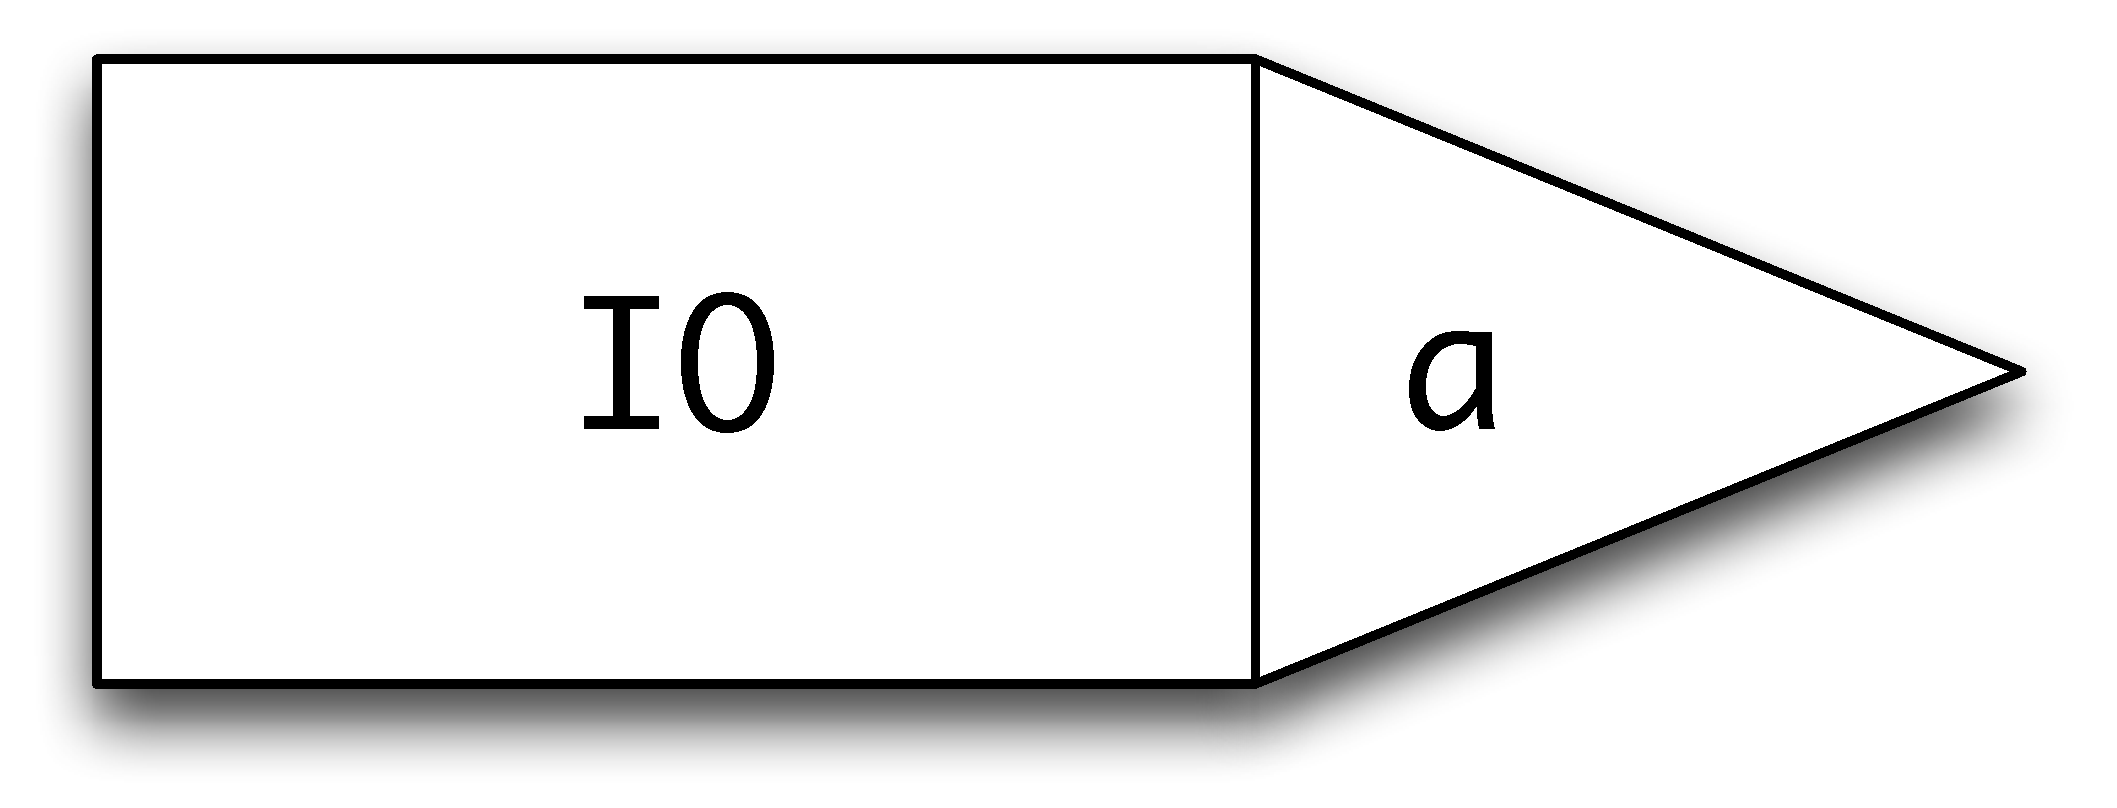
\includegraphics[height=1.2cm]{Pictures/Monad1.pdf}
\end{center}
with a \textbf{function}
taking the result of this (of type \texttt{a}) into an \texttt{IO b}, that is 
an object of type \texttt{a -> IO b},
\begin{center}
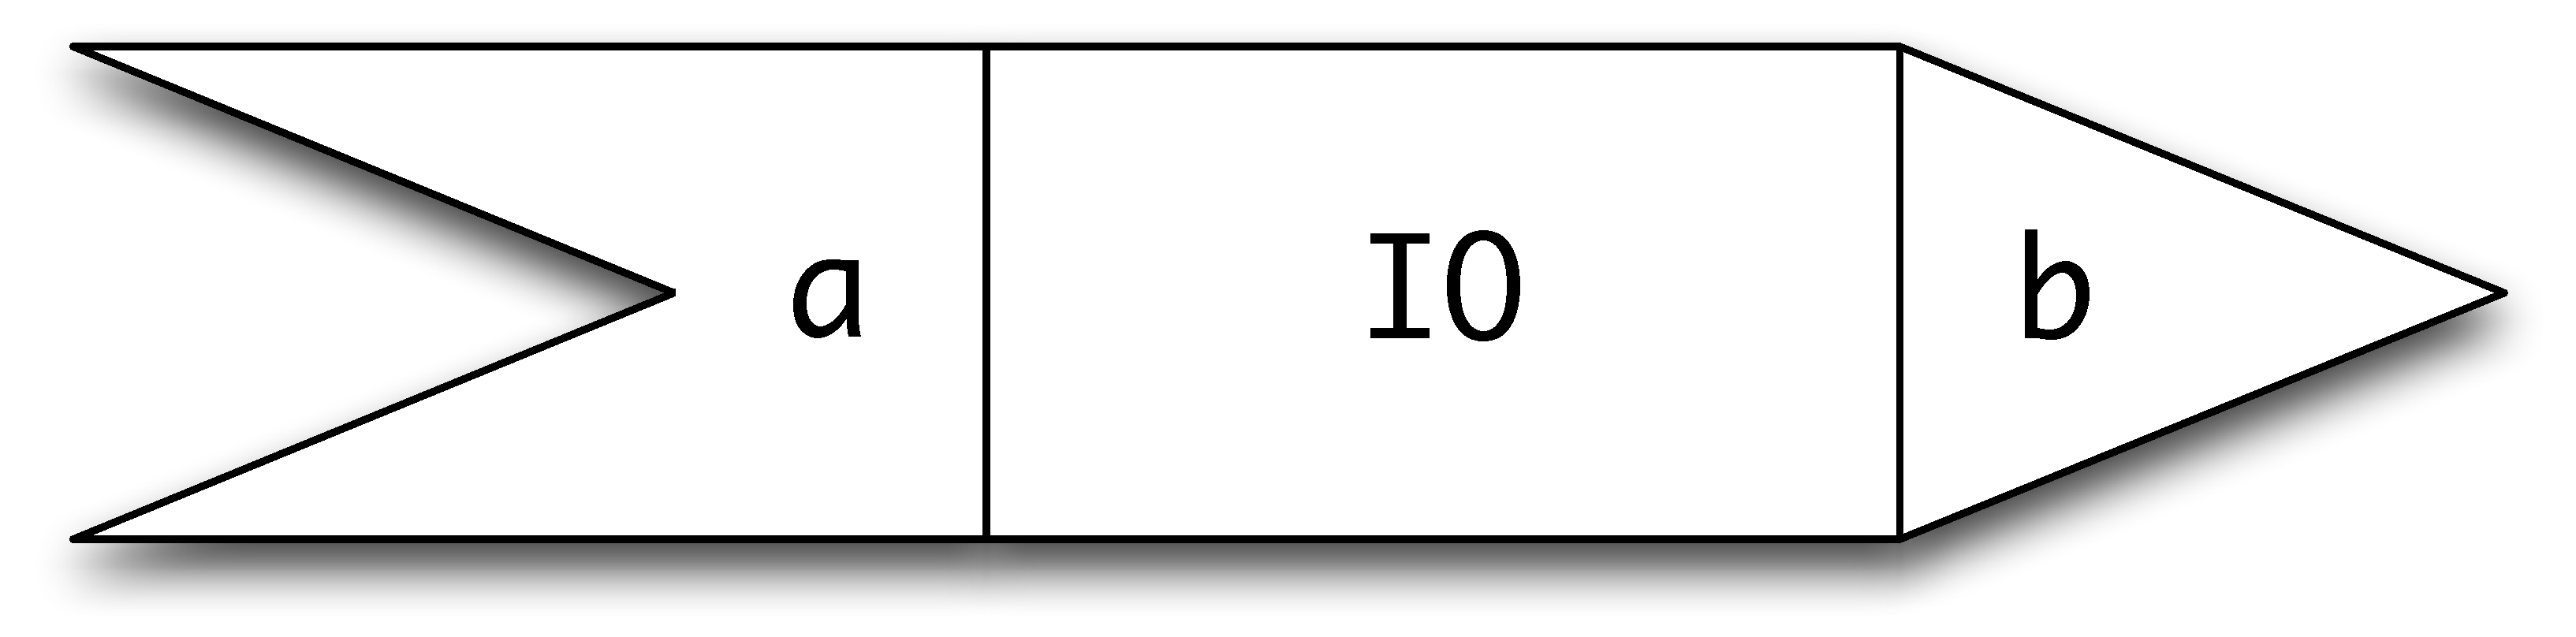
\includegraphics[height=1.2cm]{Pictures/Monad2.pdf}
\end{center}
We can join them together, passing the result of the first as an argument to
the second, thus:
\begin{center}
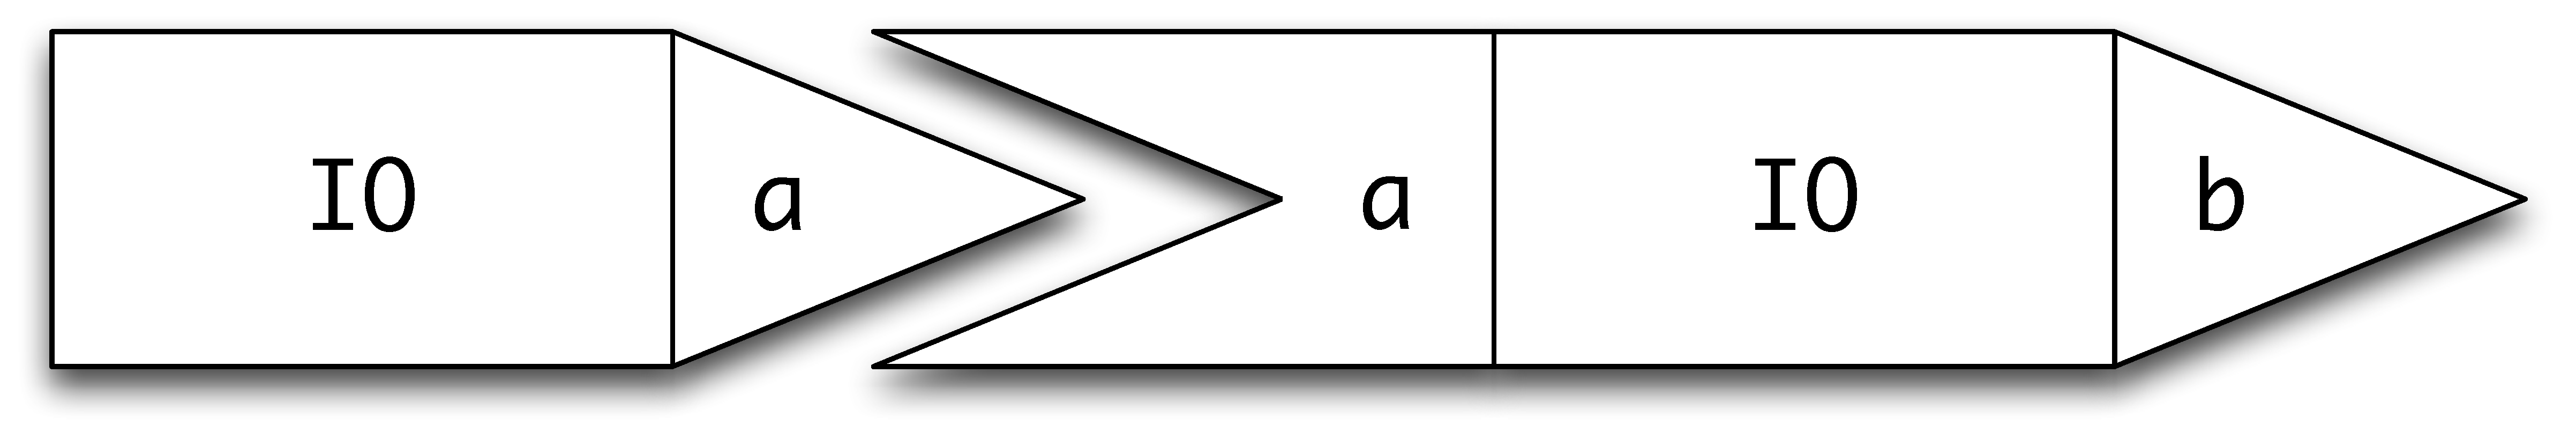
\includegraphics[height=1.2cm]{Pictures/Monad3.pdf}
\end{center}
The result of putting them together is something which does some I/O before
returning a value of type \texttt{b}:
\begin{center}
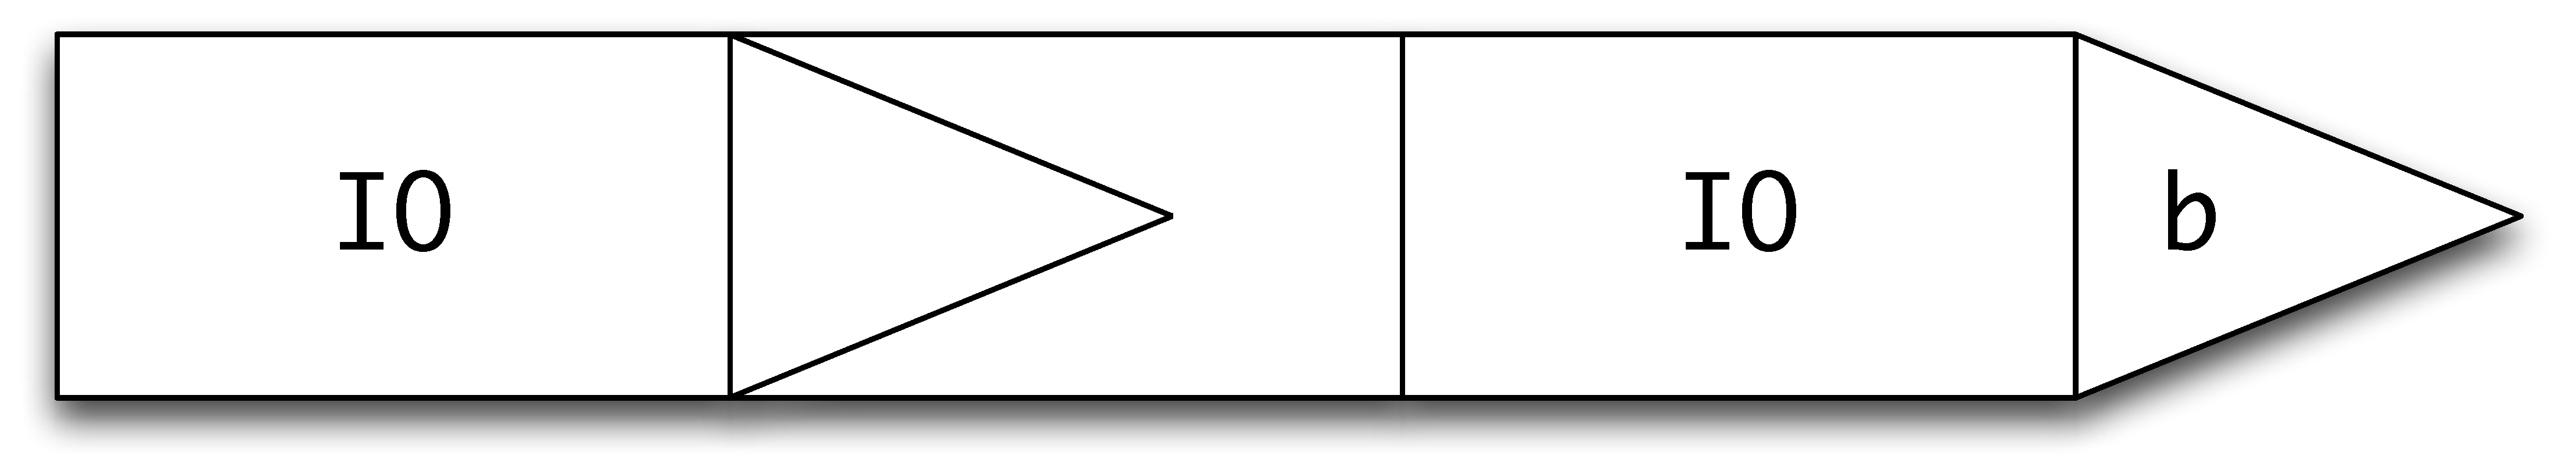
\includegraphics[height=1.2cm]{Pictures/Monad4.pdf}
\end{center}
in other words, an object of type \texttt{IO b}. 

How does this relate to
the \texttt{do} notation? The bind operation, \texttt{(>>=)}, is one of the simplest possible things we can define using \texttt{do}:
\begin{alltt}
m >>= f =
    do
      res <- m
      f res
\end{alltt}
First what we do is execute \texttt{m}, which is to type \texttt{IO a}, and name its result \texttt{res}; we then pass that to the function \texttt{f}, giving \texttt{f res} ,which is of type \texttt{IO b}.

In fact we can translate \emph{every} use of \texttt{do} into calls to \texttt{(>>=)}; \texttt{do} is just \emph{syntactic sugar} to make writing IO programs more readable.
Let's look at a particular example; consider what happens in the program
\begin{alltt}\minx{addOneInt}
addOneInt :: IO ()
addOneInt 
  = do line <- getLine
       putStrLn (show (1 + read line :: Int))       
\end{alltt}
The value returned by \texttt{getLine} is called \texttt{line} and then
used in the subsequent interaction. Using \texttt{(>>=)} we have to
sequence the interaction with a function expecting an argument of type
\texttt{String}, so we write
\begin{alltt}
addOneInt 
  = getLine >>= \bs{line} ->
    putStrLn (show (1 + read line :: Int))       
\end{alltt}
where recall that \texttt{\bs{x} -> e} is the function which takes the
parameter \texttt{x} to result \texttt{e}, so here the parameter is
called \texttt{line}, and used just as above. More complex examples
are translated in a similar way. 

As you can see from this simple example, using \texttt{(>>=)} makes programs more difficult to read and understand: the \texttt{do} notation highlights the essential features of I/O programming:
\begin{titemize}
\item sequencing operations, and,
\item binding the results of statements for use later on in the program.
\end{titemize}
and gives a readable and comprehensible way of writing these programs within Haskell.

We'll continue to use the
\texttt{do} notation, but will keep in mind that it essentially boils down to the existence of a
function \texttt{(>>=)} which does the work of sequencing I/O programs, and binding their results for future use.

\begin{exerciseone}
\item
Repeat some of the earlier examples and exercises using the \texttt{>>=}
operator instead of a \texttt{do} expression.
\index{I/O|)}
\end{exerciseone}

\section{Monads: languages for functional programming}
\label{monadFP}
\index{monad|(}


The \texttt{do} notation allows us to write \emph{programs} which perform I/O while calculating results; as we discussed in the last section, all we need to support the \texttt{do} notation is to have the `bind' function and `return' functions:
\begin{alltt}\minx{return}\index{\symbol{62}\symbol{62}\symbol{61}@\texttt{\symbol{62}\symbol{62}\symbol{61}}}
(>>=) :: IO a -> (a -> IO b) -> IO b
return :: a -> IO a
\end{alltt} 
The \texttt{IO} types give one kind of program which we can describe with the \texttt{do} notation, but there are other kinds of program we might want to write in a similar way, such as
\begin{titemize}
\item
programs that are \emph{non-deterministic}: we can think of these as programs which return a collection of results, as a list, say;
\item
programs that might give no answer at all;
\item
programs that work by manipulating a \emph{state}: that is programs that have variables in the sense of imperative languages like Java and C;
\item
programs that raise \emph{exceptions}, and can have those exceptions handled within the program.
\end{titemize}
Well, we \emph{can} do this, so long as the types have the analogue of the bind and return functions. In other words, we need to implement functions in a particular kind of \emph{interface}, and we know from Chapter \ref{classes} that this is given in Haskell by the \texttt{Monad} class, like this:
\begin{alltt}\minx{Monad}
class Monad m where
  (>>=)  :: m a -> (a -> m b) -> m b
  return :: a -> m a
\end{alltt}
Once we have an instance of this class we can use the \texttt{do} notation over the type. 

Let's look at the example of programs that might might give no answer, the second in the list of examples above. We looked at these in Section \ref{progErrs} where we saw that the \texttt{Maybe} type was a good model for values including a potentially absent result:
\begin{alltt}\minx{Maybe}\index{monad!\texttt{Maybe}}
data Maybe a = Nothing | Just a
\end{alltt}
and we developed a number of functions which worked with \texttt{Maybe} types to transmit errors through the code. Alternatively we can use the \texttt{do} notation, because we have this \texttt{instance} for \texttt{Monad}:
\begin{alltt}
instance Monad Maybe where
  (Just x) >>= k  =  k x
  Nothing  >>= k  =  Nothing
  return x        =  Just x
\end{alltt}
so that we get this behaviour using \texttt{do}:
\begin{alltt}
\textsl{Prelude>} do \{ x <- Just 1; y <- Just 2; return (x+y) \}
\textsl{Just 3}
\textsl{Prelude>} do \{ x <- Just 1; y <- Nothing; return (x+y) \}
\textsl{Nothing}
\textsl{Prelude>} do \{ x <- Nothing; y <- Just 2; return (x+y) \}
\textsl{Nothing}
\end{alltt}
where we are using the braces `\{', `\}' and explicit separator `:' to put the statements in the \texttt{do} program on a single line, as first introduced in Chapter \ref{writingProgs}. In a similar way, lists form a monad:
\begin{alltt}\index{monad!list}
instance Monad [] where
  xs >>= f  = concat (map f xs)
  return x  = [x]
\end{alltt} 
and we can use \texttt{do} notation over lists, like this:
\begin{alltt}
\textsl{Prelude>} do \{ x <- [1,2]; y <- [3,4]; return (x+y) \}
\textsl{[4,5,5,6]}
\end{alltt}
From this example we can see that lists model \emph{non-deterministic} computation: each of \texttt{x} and \texttt{y} have two possible values, and that gives four possibilities for \texttt{(x+y)}. The definition of \texttt{(>>=)} over lists reflects this: \texttt{f} is applied to all the possibilities in \texttt{xs} and the results are concatenated together.

In the next section we fill in some of the formalities about monads, but this latter section can be skipped on first reading, if you wish. We then look at some more examples of monads.

\beware{Why `monad'?}{\index{monad!terminology}
Why is this type class called `monad'? The name originates in category theory, which was used by Eugenio Moggi to build mathematical models of different kinds of computations. However, that doesn't mean that you need to learn category theory to use them, any more than you need to understand the intricacies of modern microprocessors to use your computer! Understanding that the \texttt{do} notation gives sequencing and binding (or naming) is all you need to understand to get started.}

\subsection*{Monads, formally}
\index{monad!definition}\minx{>>}

\index{\symbol{62}\symbol{62}\symbol{61}@\texttt{\symbol{62}\symbol{62}\symbol{61}}}
\minx{return}
A monad is a family of types \texttt{m a}, based on a polymorphic type
constructor \texttt{m}, with functions \texttt{return}, \texttt{(>>=)} and
\texttt{(>>)}:
\begin{alltt}
class Monad m where
  (>>=)  :: m a -> (a -> m b) -> m b
  return :: a -> m a
  (>>)   :: m a -> m b -> m b
\end{alltt}
This is an example of a \textbf{class}, whose instances are
\textbf{type constructors} -- that is functions which build types from
types -- rather than types. Examples of type constructors are `list',
written \texttt{[]} in Haskell, 
and \texttt{IO} as we have seen already.

The definition of \texttt{Monad} also contains a default declaration for \texttt{>>}:
\begin{alltt}
m >> k = m >>= \bs{}\_ -> k 
\end{alltt}
From this definition it can be seen that \texttt{>>} acts like \texttt{>>=}, except that the value
returned by the first argument is discarded rather than being passed to the second argument.

In order properly to be a monad, the functions \texttt{return} and \texttt{(>>=)}
should have some simple properties. Informally we can state the requirements
like this:
\begin{itemize}
\item
The operation \texttt{return x} should simply return the value
\texttt{x}, without any additional computational effect, such as input
or output in the case of the \texttt{IO} monad.
\item
The sequencing given by \texttt{>>=} should be irrelevant of the way
that expressions are bracketed.
\end{itemize}
The laws are much clearer when stated in terms of a derived operator,
\texttt{>=>}, prnounced `fish', that is defined in \texttt{Control.Monad}:
\index{\symbol{62}\symbol{64}\symbol{62}@\texttt{\symbol{62}\symbol{64}\symbol{62}}}
\begin{alltt}
(>=>) :: Monad m => (a -> m b) ->
                    (b -> m c) ->
                    (a -> m c)

f >=> g = \bs{x} -> (f x) >>= g
\end{alltt} 
This operator generalizes function composition\footnote{In category theory, this
operation is called \textbf{Kleisli composition}\index{Kleisli composition}.} \index{function composition}
in that it composes
objects 
\begin{center}
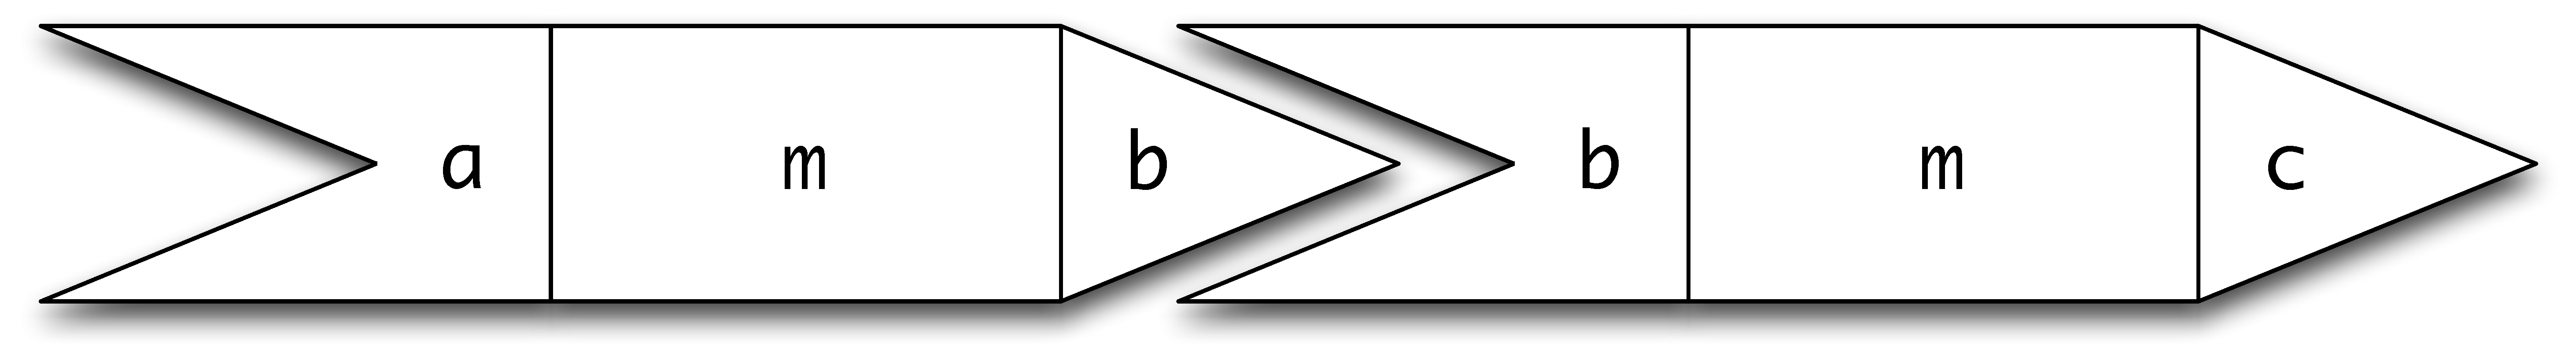
\includegraphics[height=1.2cm]{Pictures/Monad5.pdf}
\end{center}
to give
\begin{center}
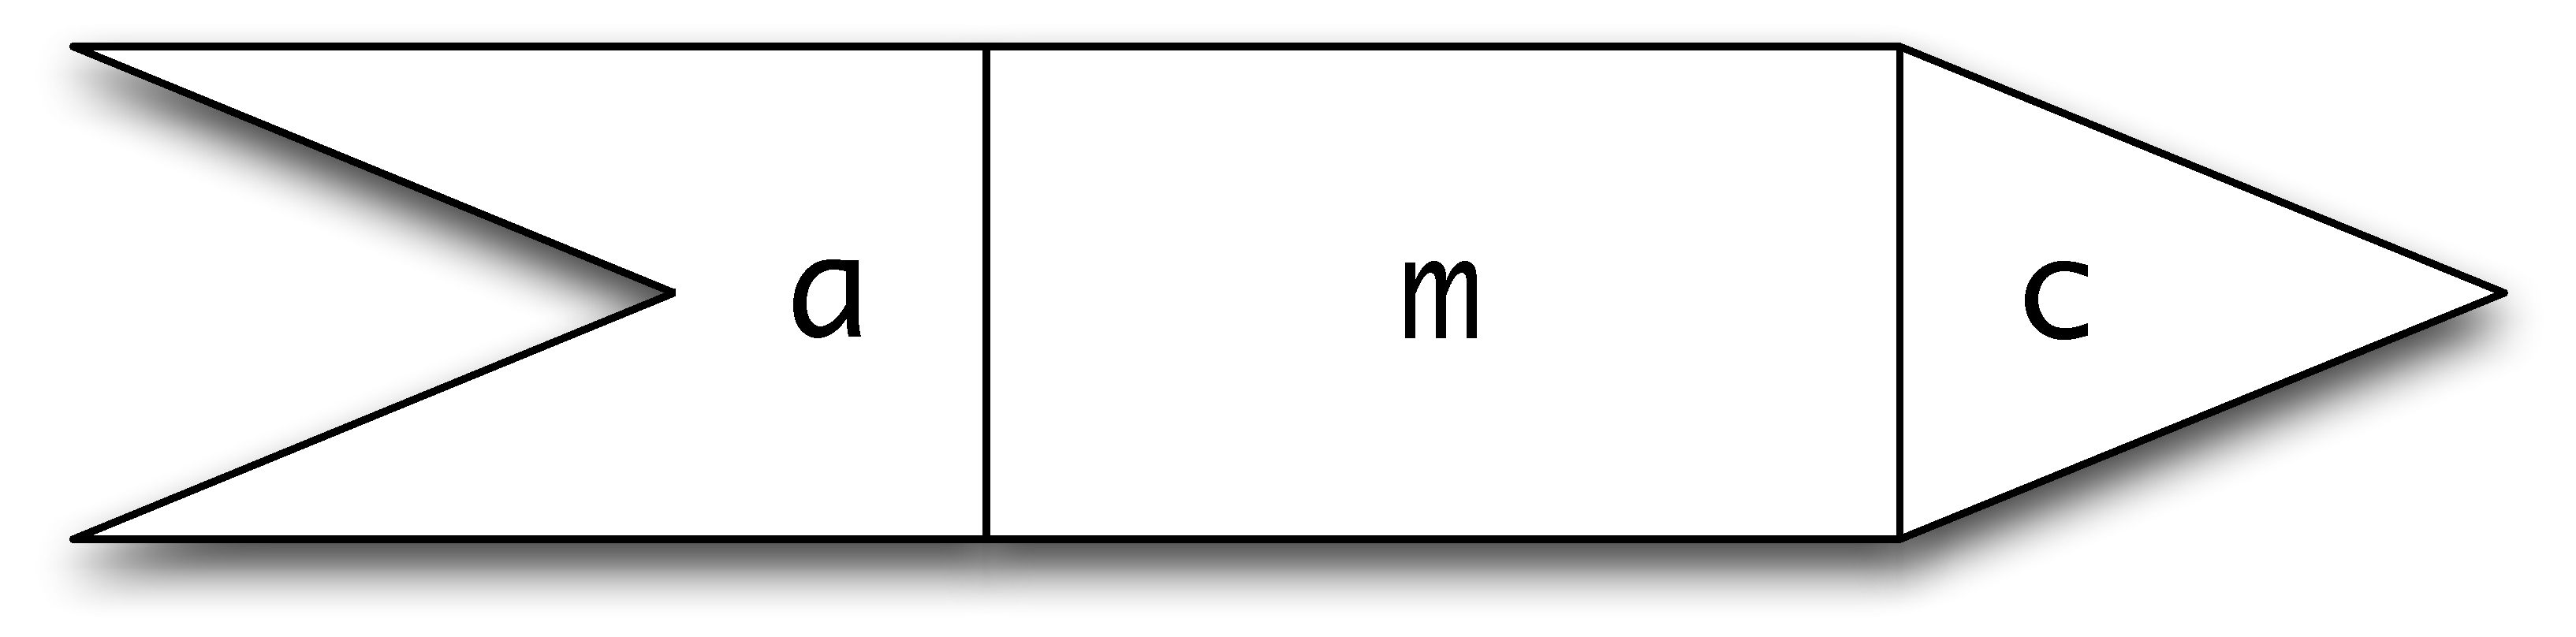
\includegraphics[height=1.2cm]{Pictures/Monad6.pdf}
\end{center}
Note also that \texttt{return} is of this shape, as its type is
\texttt{a -> m a}. 

Now we can state formally the rules that the operations of
a monad should satisfy. \index{monad!properties}
First,
\texttt{return} is an \textbf{identity}\index{identity} for the operator \texttt{>=>}:
\begin{alltt}
return >=> f = f\hfill(M1)
f >=> return = f\hfill(M2)
\end{alltt}
and the operator \texttt{>=>} should be \textbf{associative}:\index{associativity}
\begin{alltt}
(f >=> g) >=> h = f >=> (g >=> h)\hfill (M3)
\end{alltt}
The derived sequencing operator, \texttt{>>}\minx{>>}, is also associative.

Of course, there is no way that we can make the requirements \texttt{(M1)}--\texttt{(M3)} 
a part of
the Haskell definition of \texttt{Monad}. 
We can also restate the rules in terms of
\texttt{do}, since, as we saw earlier,
\begin{alltt}
m >>= f  =  do \{ x <- m; f x \}
\end{alltt}
The first two rules become
\begin{alltt}
do \{ y <- return x; f y \} =  f x
do \{ x <- m; return x \}   =  m
\end{alltt}
and the third is implicit in the fact that the \texttt{do}
construct is associative.

\subsection*{Adding failure, \texttt{MonadFail}}
This type class adds a function marking that a computation has failed, \texttt{fail}, to an existing monad.
\begin{alltt}\minx{MonadFail}\minx{fail}
class Monad m => MonadFail m where
  fail   :: String -> m a
\end{alltt}
\item
The value \texttt{fail} \texttt{s} corresponds to a computation which
\textbf{fails}, giving the error message \texttt{s}. \index{monad!failure in (\texttt{fail})}

The definition of \texttt{MonadFail} also contains a default declaration for \texttt{fail}
\begin{alltt}
fail s = error s
\end{alltt}

\begin{exercises}
 

\item
Show that lists and the \texttt{Maybe} type are instances of \texttt{MonadFail}. Hint: in both cases the \texttt{String} argument is ignored.

\item
Once a computation has failed, it cannot be ``unfailed'' as it were. As a law this is expressed as \texttt{fail s >>= f  =  fail s}. Show that this rule holds for the instances of \texttt{MonadFail} that you defined in the previous exercise.


\end{exercises}

\subsection*{Some more examples}
\index{monad!examples}

Now we have seen the definition of what it means to be a monad, with or without failure, we look at some more examples of monads in Haskell.



\subsubsection*{The parsing monad}
\index{parsing!monad}
\index{monad!parsing}


A more substantial example is given by parsing, where we can show that
\texttt{Parse a} is a monad. To make a formal declaration of this we
need to wrap it in a \texttt{newtype} constructor, \texttt{MP},
which clutters the definition a bit.
\begin{alltt}
newtype MP a b = MP \{ mp :: (Parse a b) \}

instance Monad (MP a) where
  return x = MP (succeed x)
  (MP pr) >>= f 
    = MP (\bs{st} -> concat [ mp (f x) rest | (x,rest) <- pr st ])

instance MonadFail (MP a) where
  fail s   = MP none
\end{alltt}
The crux of the definition of \texttt{(>>=)} is like that of
\texttt{(>*>)} -- a parse is done by one parser, \texttt{pr}, and the remains of the
input are passed to a second parser \texttt{f}, here dependent on the result of the
first parse, and so a result of the first parse, \texttt{x}, is passed
to \texttt{f} to give a second parser, which is applied to the remaining
input, \texttt{rest}.

How does the monadic approach to parsing look in practice? Let's go back to the calculator example, and in particular the definition of \texttt{opExpParse} in Section \ref{parsing}, page \pageref{opExpParse}. If we redefine it monadically, we get
\begin{alltt}
opExpParseM :: MP Char Expr
opExpParseM =
    do
      tokenM '('
      e1 <- parseExprM 
      bop <- spotM isOp
      e2 <- parseExprM
      tokenM ')'
      return (Op (charToOp bop) e1 e2)
\end{alltt}
where \texttt{tokenM} is the monadic equivalent of \texttt{token}, and so forth. How do the definitions differ? It is mainly in the handling of the results: in the earlier treatment we built the results into a nested tuple, gathering a result for each step whether or not we needed it, and then passed the tuple to a function, via \texttt{build}. The approach here has the advantage that
\begin{titemize}
\item
we only name the results of the sub-parses that we need, and
\item
we can build the final result directly, using these names, rather than having to use a function to re-jig the tuple into the value we want.
\end{titemize} 
The disadvantage of the non-monadic approach is reminiscent of the discussion of `point-free' programming on page \pageref{pointfree}: under both we combine functions, when the judicious use of names (of variables, of intermediate results) make the program substantially easier to read, write and understand.

\subsubsection*{The identity monad}
\index{monad!identity}

The identity monad, which takes a type to itself, is the simplest
example of a monad, with the definitions
\begin{alltt}
x >>= f = f x 
return = id
\end{alltt}
In order for this to be a legal Haskell definition we need to define the identity type constructor, and, within Haskell 2010, any instance declaration needs to be for a \texttt{data} type, \texttt{newtype} or primitive type. So, we define, as in \texttt{Control.Monad.Identity},   
\begin{alltt}
newtype Identity a = Identity { identity :: a }
\end{alltt}
where the constructor \texttt{Identity} `wraps' the value up, and the field name, \texttt{identity} is used to `unwrap' them.. Now we can define the instance itself,
\begin{alltt} 
instance Monad Identity where
    (Identity x) >>= f = f x          --  x >>= f = f x 
    return a           = Identity a   --  return = id 
\end{alltt}
We can then run things in this monad, if we give a \texttt{Show} instance for \texttt{Identity}
\begin{alltt}
instance Show a => Show (Identity a) where
    show (Identity x) = show x
\end{alltt}
as in this example, which also shows how we can give multi-line input to GHCi interactively.
\begin{alltt}
\textsl{*UseMonads>} :\{
\textsl{*UseMonads}| do \{ x <- return 'c' :: Identity Char;
\textsl{*UseMonads}|      y <- return 'd';
\textsl{*UseMonads}|      return [x,y] \}
\textsl{*UseMonads}| :\}
\textsl{"cd"}
\end{alltt}
Computationally, this monad represents the trivial state in which no
actions are performed, and values are returned immediately.




\subsubsection*{The state monad}
\index{monad!state}

Later in this chapter we will give an example of a \textbf{state} monad, 
\texttt{State a b}. An operation of this type can change the state (of type 
\texttt{a}) before returning
a value of type \texttt{b}.





\subsection*{Some standard functions and the \texttt{Functor} class}

There is a set of standard functions over monads, defined in \texttt{Control.Monad}; we just look at two of these here. Their types should be
familiar from the list case
\begin{alltt}\minx{fmap}\minx{join}
fmap :: Monad m => (a -> b) -> m a -> m b
join :: Monad m => m (m a) -> m a
\end{alltt}
and their definitions are
\begin{alltt}
fmap f m 
  = do x <- m 
       return (f x)
join m  
  = do x <- m
       x
\end{alltt}
Over lists these functions are called \texttt{map} and \texttt{concat};
many of the properties of \texttt{map} and \texttt{concat} over lists lift to these
functions. For instance, we can show using properties \texttt{(M1)} to \texttt{(M3)}
that for all \texttt{f} and \texttt{g}
\begin{alltt}
fmap (f.g) = fmap f . fmap g\hfill(M4)
\end{alltt}
In fact, \texttt{fmap} is defined over a wider set of types that monads, and it is the function that characterises the \texttt{Functor}\minx{Functor} class that we saw earlier:
\begin{alltt}
class Functor f where
  fmap :: (a -> b) -> f a -> f b
\end{alltt}
Example instances of \texttt{Functor} which are not monads include \texttt{(a,a)}, \texttt{([a],[a])} and \texttt{Tree a} (from the next section).

\begin{exercises}

\item
Show that sets and binary trees
can be given a monad structure, as can the type:
\begin{alltt}
data Error a = OK a | Error String
\end{alltt}

\item
For the monads \texttt{Id} , \texttt{[]} and \texttt{Maybe} prove the rules 
\texttt{(M1)} to \texttt{(M3)}. Also show that
these rules hold for your implementations in the
previous exercise.

\item
Prove the property \texttt{(M4)} using the laws \texttt{(M1)} to \texttt{(M3)}.

\item 
Prove the following properties using the monad laws:
\begin{alltt}
join . return = join . fmap return
join . return = id
\end{alltt}

\item
Can you define a different monad structure over lists from that given above?
Check that your definition has properties \texttt{(M1)} to \texttt{(M3)}.

\item
Write down the definitions of \texttt{map} and \texttt{join} over lists
using list comprehensions. Compare them with the definitions of
\texttt{fmap} and \texttt{join} given in the \texttt{do} notation in this section.

\item
Re-implement the parser for the calculator using the \texttt{do}
construct (based on \texttt{>>=}) 
rather than \texttt{(>*>)} and \texttt{build}. Contrast the two
approaches.

\item
Show that the type functions \texttt{(a,a)}, \texttt{([a],[a])} and \texttt{Tree a} are instances of \texttt{Functor}.

\end{exercises}

\section{Example: monadic computation over trees}
\index{monad!trees}
\label{monadicTrees}

We now illustrate how computations over the type of 
\begin{alltt}
data Tree a = Nil | Node a (Tree a) (Tree a)\minx{Tree}
\end{alltt}
can be given a monadic structure. We first look at a simple example, and then
we look at a rather more realistic one. 

We see that with a monadic approach the top-level
structure of the two solutions 
is exactly the same. This structure guides the way that we build the
implementation of the second example, as we shall see.

The moral of these examples is
that monads provide an important structuring mechanism for program
construction, as they encourage a \textbf{separation of concerns}. The
top-level structure of the computation is given in terms of a
monad whose specific properties are only touched upon. Within the monad itself
is the appropriate computational behaviour to, for example, 
maintain a state or to perform some
IO (or both); the particular sequencing operation of the monad will
ensure that values are passed between the parts of the program in an
appropriate way.

This separation of concerns comes into its own when changes are required
in the details of the computation: it is usually possible to change the monad
implementing a computation with at most minimal changes required at the
top level. This is in stark contrast to a non-monadic computation in
which data representations are visible: a wholesale restructuring is
often required in such a situation.

\subsection*{Summing a tree of integers}

Suppose we are asked to give the sum of a tree of integers,
\begin{alltt}
sTree :: Tree Integer -> Integer
\end{alltt}
A direct recursive solution is
\begin{alltt}\minx{sTree}
sTree Nil            = 0
sTree (Node n t1 t2) = n + sTree t1 + sTree t2
\end{alltt}
In writing this we give no explicit sequence to the calculation of the sum: we
could calculate \texttt{sTree t1} and \texttt{sTree t2} one after the other, or
indeed in parallel. How might a monadic solution proceed?
\begin{alltt}
sumTree :: Tree Integer -> St Integer\minx{sumTree}
\end{alltt}
where \texttt{St} is a monad which we have yet to define. In the \texttt{Nil} case,
\begin{alltt}
sumTree Nil = return 0
\end{alltt}
while in the case of a \texttt{Node} we calculate the parts in a given order:
\begin{alltt}
sumTree (Node n t1 t2)\hfill(sumTree)\label{sumTree}
  = do num <- return n
       s1  <- sumTree t1
       s2  <- sumTree t2
       return (num + s1 + s2)
\end{alltt}
How is the definition structured? We put the operations in sequence, using
\texttt{do}. First we \texttt{return} the value \texttt{n}, giving it the 
name \texttt{num}. Next we calculate \texttt{sumTree t1} and \texttt{sumTree t2}, naming 
their results \texttt{s1} and \texttt{s2}. Finally we \texttt{return} the result, which
is the sum \texttt{num+s1+s2}. 

Now, since all we are doing here is calculating values and not trying to do
any I/O or other side-effecting operation, we make the monad 
\texttt{St} the {\em identity\/} monad \texttt{Identity} which we mentioned
earlier, so we have
\begin{alltt}
sumTree :: Tree Integer -> Identity Integer
\end{alltt}
There is a similarity between the definition \texttt{(sumTree)} and an
imperative program, bearing in mind that \texttt{do} performs a sequencing and
\texttt{j <- ...} gives (or assigns) a value to \texttt{j}. In an imperative
setting, we might well write 
\begin{alltt}
num := n ;
s1  := sumTree t1 ;
s2  := sumTree t2 ;
return (num + s1 + s2) ;
\end{alltt}
where `\texttt{num :=}' corresponds to the `\texttt{<-}' and \texttt{do} puts a 
sequence of commands one after the other, as does the semi-colon. Remember, though, that this is a \emph{single-assignment} language, so that \texttt{num}, \texttt{s1} and so on are names not variables!
\index{monad!and imperative programming}
\index{imperative programming!and monads}

To give a function of type \texttt{Tree Integer -> Integer} we compose with the
\texttt{identity} function to give
\begin{alltt}
identity . sumTree
\end{alltt}
where
\begin{alltt}
identity :: Identity a -> a
identity (Identity x) = x
\end{alltt}
takes the wrapper off an element \texttt{Identity x} to give the element
\texttt{x}.
In the next section we tackle a more complex problem, but see the same monadic
structure repeated.

\subsection*{Using a state monad in a tree calculation}
\index{monad!state}

Building on the experience of the last section in defining \texttt{sumTree} we
tackle here a rather more tricky problem. We want to write a function
\begin{alltt}
numTree :: Eq a => Tree a -> Tree Integer
\end{alltt}
so that given an arbitrary tree we transform it to a tree of integers in which
the original elements are replaced by natural numbers, starting from \texttt{0}.
An example is given in Figure \ref{treeTrans}.
The same element has to be replaced by the same number at every occurrence,
and when we meet an as-yet-unvisited element we have to find a `new' number to
match it with.

\begin{figure}[t]
\begin{center}
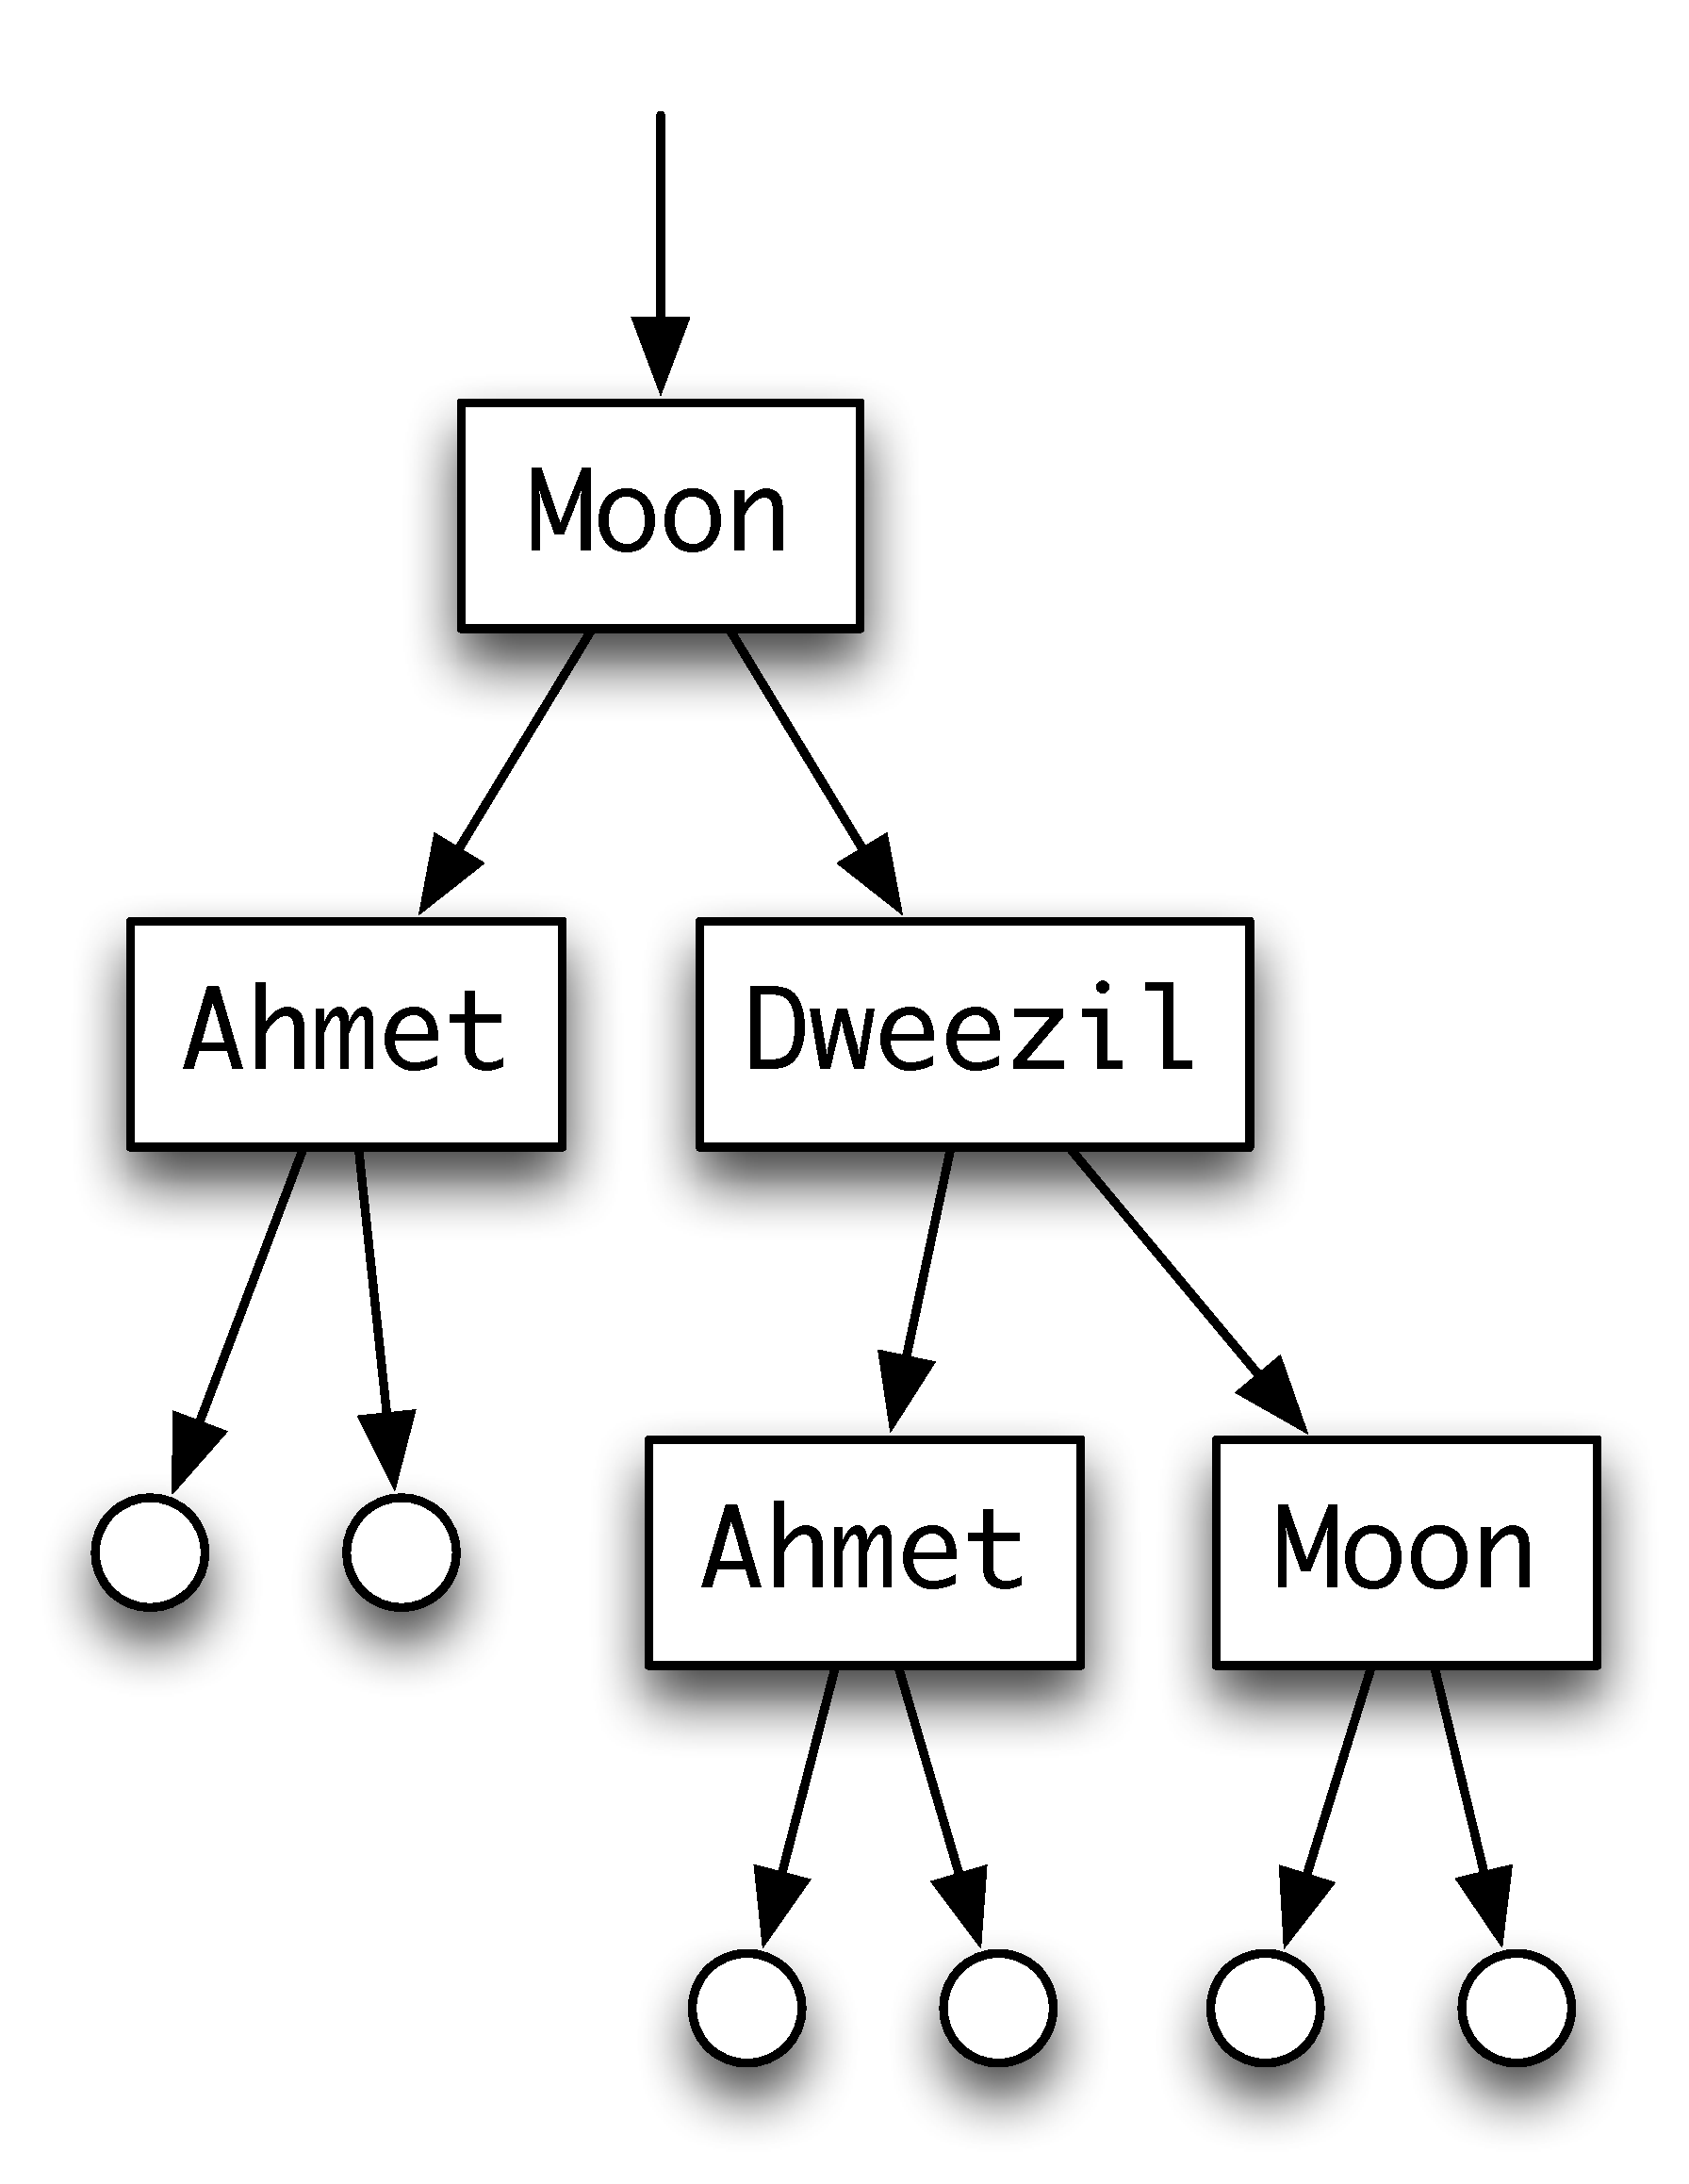
\includegraphics[height=6cm]{Pictures/TreeBefore.pdf}\hspace*{1cm}
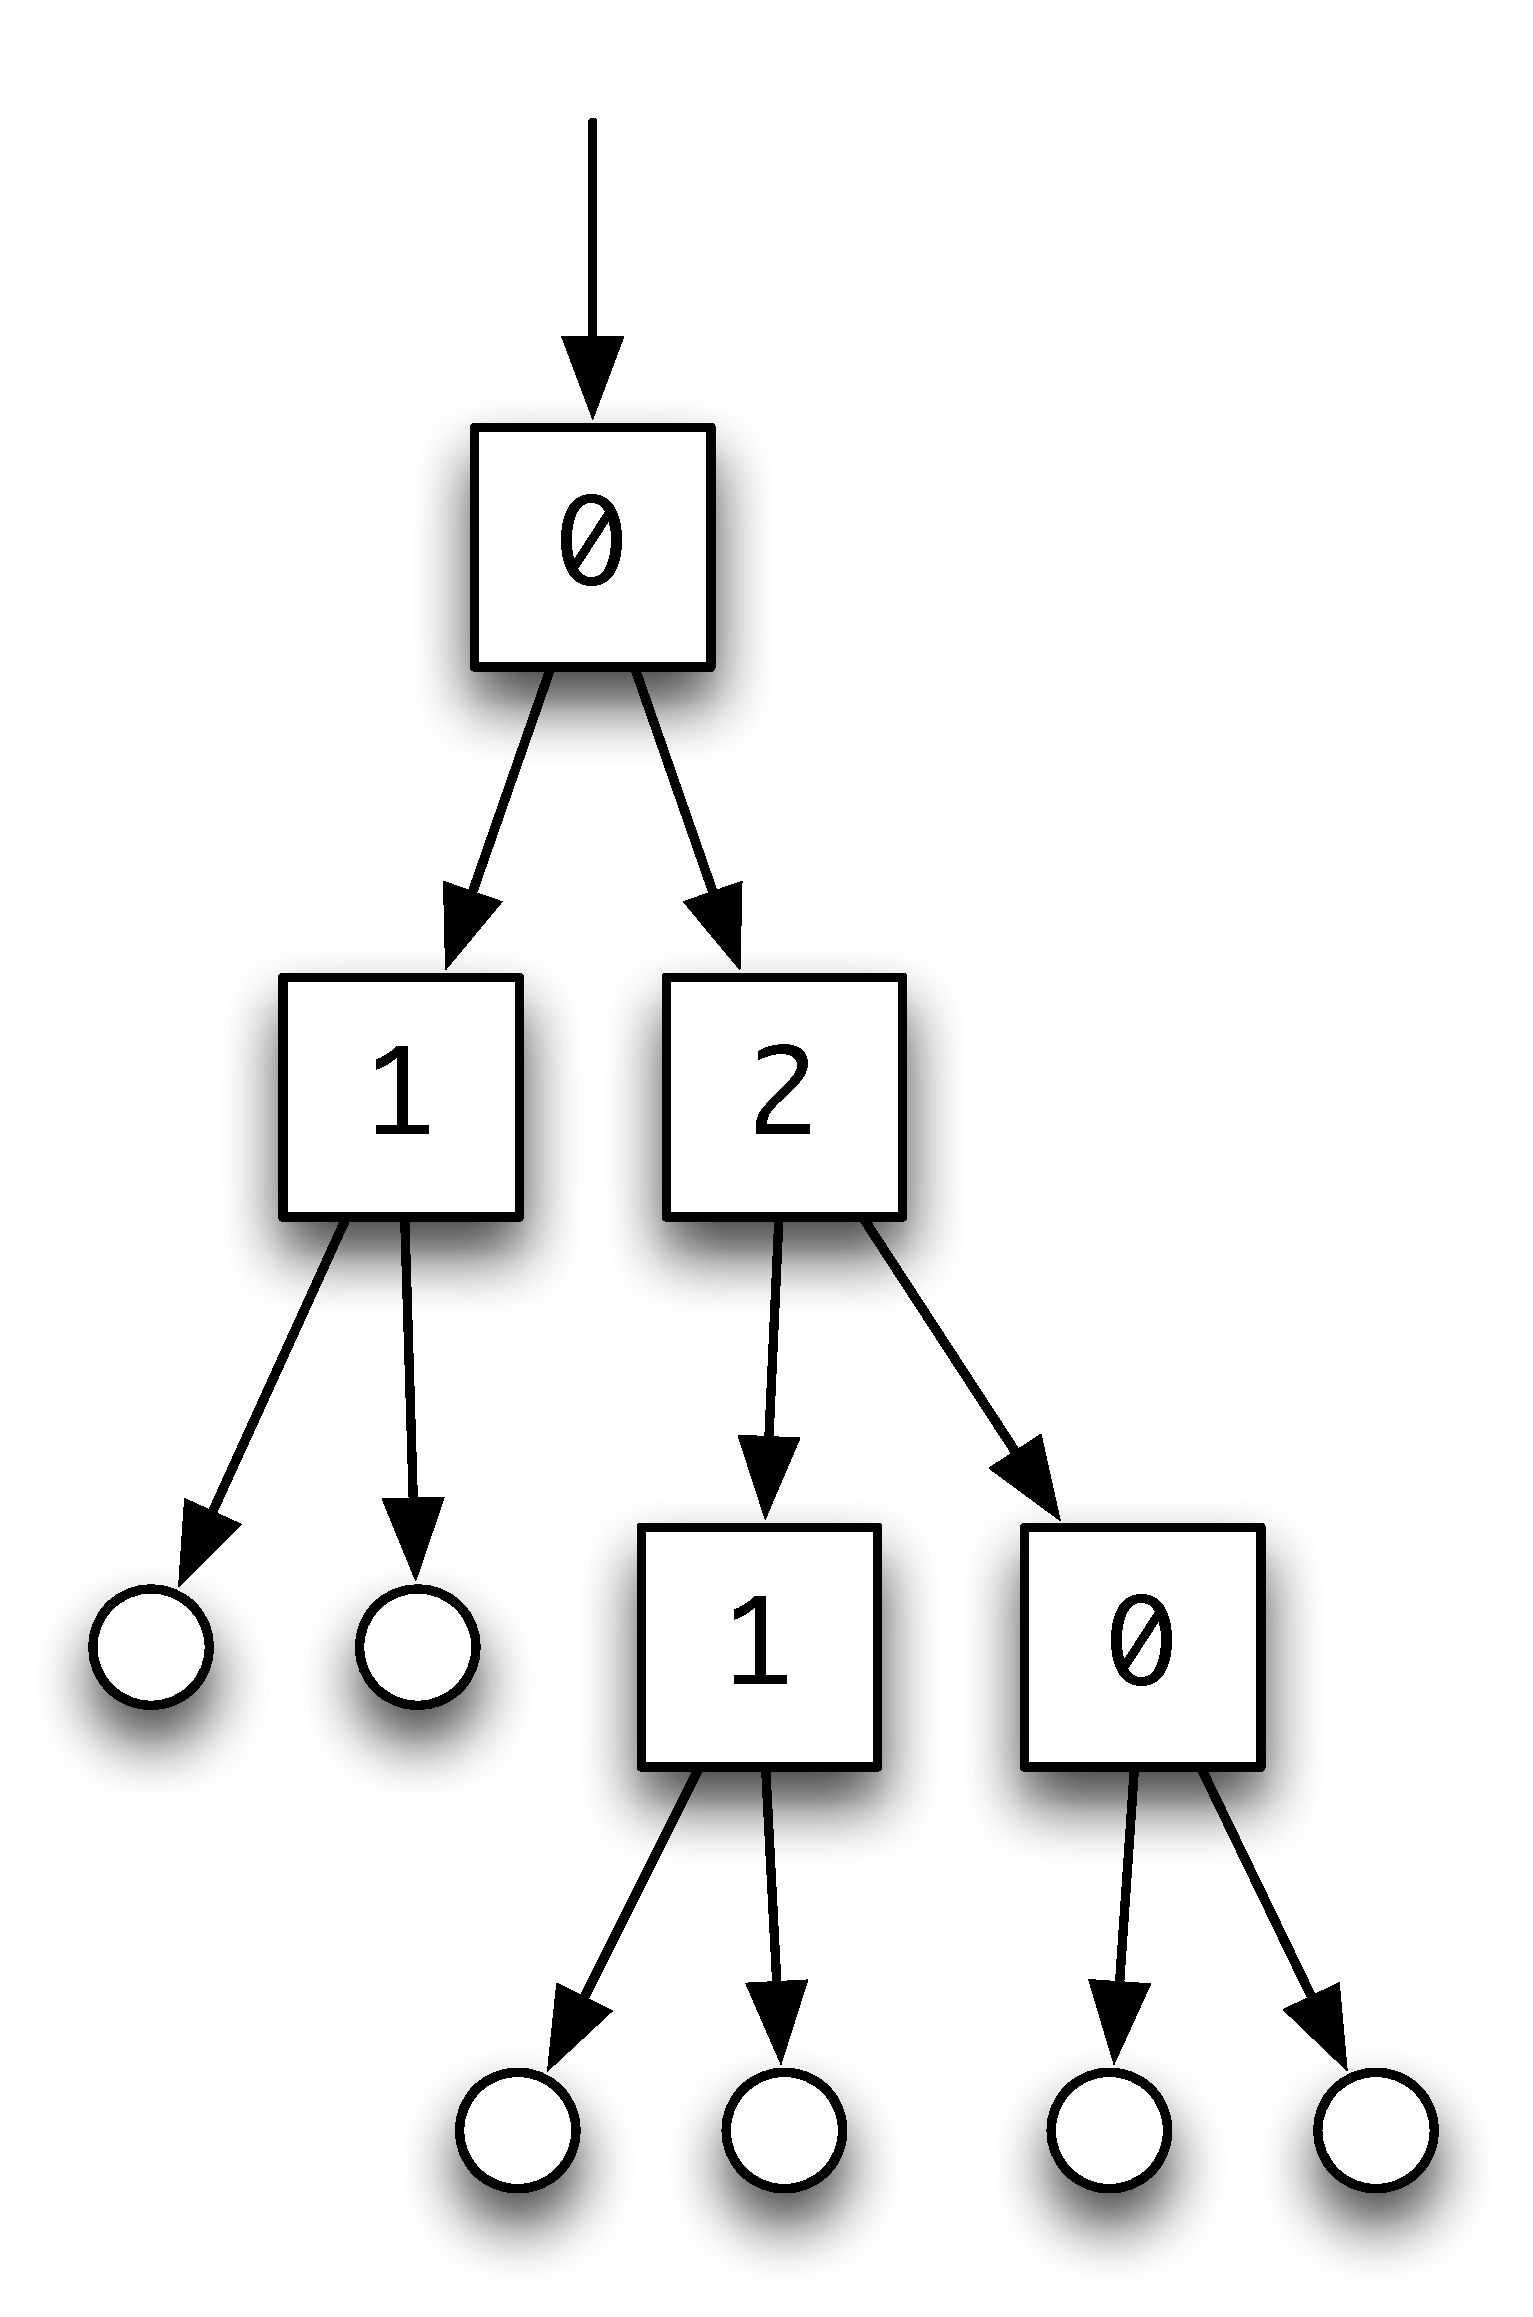
\includegraphics[height=6cm]{Pictures/TreeAfter.pdf}
\end{center}
\caption{Replacing the elements of a tree with natural numbers.}
\label{treeTrans}
\end{figure}

\subsubsection*{Describing the calculation}


How does our definition appear? We give the function a type,
\begin{alltt}\minx{numberTree}
numberTree :: Eq a => Tree a -> State a (Tree Integer)
\end{alltt}
in which the monad \texttt{State a} will have to carry about enough information
to allow us to replace the elements in the correct way. The structure of the
program then is
\begin{alltt}
numberTree Nil = return Nil

numberTree (Node x t1 t2)\hfill(numberTree)
  = do num <- numberNode x
       nt1 <- numberTree t1
       nt2 <- numberTree t2
       return (Node num nt1 nt2)
\end{alltt}
The structure here is exactly the same as that of \texttt{(sumTree)} on
page \pageref{sumTree}; we perform
the operations on the components \texttt{x}, \texttt{t1} and \texttt{t2} (for the
subtrees we use recursion) and then combine them in the result 
\texttt{(Node num nt1 nt2)}.

What else do we have to define to give the result? We need to identify the
monad \texttt{State a} and to define the function which replaces an individual
\minx{State}
entry, 
\begin{alltt}
numberNode :: Eq a => a -> State a Integer
\end{alltt}
We now have to think about the implementation of the monad. We have called it
\texttt{State} since it keeps a record of the state, that is of which values are
associated with which numbers. This we do in a table:
\begin{alltt}\minx{Table}
type Table a = [a]
\end{alltt}
where the table \texttt{[True,False]} indicates that \texttt{True} is associated
with \texttt{0} and \texttt{False} with \texttt{1}.

\subsubsection*{The \texttt{State} monad}

What then is the state monad? It consists of functions
\begin{alltt}\minx{State}
data State a b = State (Table a -> (Table a , b))
\end{alltt}
which, after we strip off the constructor \texttt{State},
we can think of as taking the state {\em before\/} doing the operation
to the state {\em after\/} the operation, together with its result. In other
words, we return a value of type \texttt{b}, but perhaps we change the value of
the state of type \texttt{Table a} as a side-effect.

Next we have to define the two monad operations.
\begin{alltt}
instance Monad (State a) where
\end{alltt}
To \texttt{return} a value, we leave the state
unchanged.
\begin{alltt}\minx{return}
  return x = State (\bs{t}ab -> (tab,x))
\end{alltt}
How do we sequence the operations?
The intended effect here is to do \texttt{st}, pass its result to \texttt{f}
and then do the resulting operation.

In more detail, to perform \texttt{st}, we pass it the table \texttt{tab}; the output of this is a
new state, \texttt{newTab}, and a value \texttt{y}. This \texttt{y} is passed to 
\texttt{f}, giving an object of type \texttt{State~a~b}; this is then performed starting
with the {\em new\/} state \texttt{newTab}. 
\begin{alltt}\index{\symbol{62}\symbol{62}\symbol{61}@\texttt{\symbol{62}\symbol{62}\symbol{61}}}
  (State st) >>= f 
    = State (\bs{t}ab -> let 
                     (newTab,y)    = st tab
                     (State trans) = f y 
                     in
                     trans newTab)
\end{alltt}
Here we can see that the operations are
indeed done in sequence, leading from one state value to the next.

\subsubsection*{Completing the definition}


This has given us the monad; all that remains is to define the function 
\texttt{numberNode}. Our definition is
\begin{alltt}\minx{numberNode}
numberNode :: Eq a => a -> State a Integer
numberNode x = State (nNode x)

nNode :: Eq a => a -> (Table a -> (Table a , Integer))
nNode x table
  | elem x table        = (table      , lookup x table)
  | otherwise           = (table++[x] , integerLength table)
    where
    integerLength = toInteger.length
\end{alltt}
If \texttt{x} is an element of \texttt{table}, we return its position in the table,
given by \texttt{lookup}; if it is not, we add it to the end of the table, and
return its position, which is the length of the table. The definition
of 
\begin{alltt}
lookup :: Eq a => a -> Table a -> Integer
\end{alltt}
is standard, and we leave it as an exercise for the reader.

\subsubsection*{Running the program}

Standing back, we can see that we have completed our definition of the
function
\begin{alltt}
numberTree :: Eq a => Tree a -> State a (Tree Integer)
\end{alltt}
but one ingredient of the solution is still needed. If we form
\begin{alltt}
numberTree exampleTree
\end{alltt}
for some \texttt{exampleTree} of the tree type, we have an object in 
\begin{alltt}
State a (Tree Integer)
\end{alltt}
In order to \emph{extract} the result of running the program, we have to write a function
\begin{alltt}
runST :: State a b -> b
\end{alltt}
This has to perform the calculation, starting with some initial table, and
return the resulting value of type \texttt{b}. The definition is
\begin{alltt}
runST :: State a b -> b
runST (State st) = snd (st [])
\end{alltt}
where we see that \texttt{st} is applied to the initial state \texttt{[]}. The result
of this is a pair, from which we select the second part, of type \texttt{b}.
Now we can define our function
\begin{alltt}
numTree :: Eq a => Tree a -> Tree Integer
numTree = runST . numberTree
\end{alltt}
which has the effect we require.

\subsubsection*{Discussion}


To conclude, we have shown how a complex calculation over a tree, 
\texttt{(numberTree)}, can be structured in exactly the same way as a simple one, 
\texttt{(sumTree)}. In the case of a tree type the advantage is tangible, but for more
complex types a monadic structure becomes almost essential if we are to follow
a computation with complicated side-effects. 

To see how much the monadic approach has tidied up the computation, it's interesting to see what the computation would look like if we passed the state around explicitly. Each function would need to take a `before' state as part of its input, and return an `after' state as part of its result. We'd then have to thread state values through the functions so that state is updated as we compute. With the monadic approach, all the explicit threading is in the definition of \texttt{(>>=)} and the rest is given by the \texttt{do} notation.

\beware{The \texttt{Control.Monad.State} module}{\minx{Control.Monad.State}
What we have presented here gives the essential idea behind the state monad in Haskell. The monad contained in \texttt{Control.Monad.State} is more complicated than the version presented here; our simplified version still gives the essential idea of a monad which threads state through a calculation.
}

\subsection*{Taking it further}\index{monad!further reading}

What we have presented here just scratches the surface of monadic programming in Haskell. We have covered the basic monads, but not looked how multiple monads -- such as state and exceptions -- can be combined into a single monad: this is done using \emph{monad transformers}, for which a number of libraries are available.

We have also not looked in any detail at monadic approaches to \emph{parsing}, beyond showing how our earlier, non-monadic, parser combinators could support a monadic view too. Most of the available Haskell parsing libraries -- which extend the basic approach in both expressivity and efficiency -- are monadic.

There are extensions to the \texttt{Monad} interface: many monads, including lists and the \texttt{Maybe} monad, have a natural notion of a sum and zero: this gives the \texttt{MonadPlus} interface. At the same time, there are various weakenings of the notion of monad, including applicative functors and arrows, each with their own advantages and disadvantages.

There is no shortage of online tutorials on monads and these other features, and other texts cover them in more detail too. A standout among these is Peyton Jones' tutorial \cite{awkwardSquad} on the `awkward squad' of monads that support IO, exceptions and other computational effects.







\index{monad|)}

\begin{exercises}

\item
Give a non-monadic definition of \texttt{numTree}, threading the state through the computation explicitly; compare your solution with the monadic version given here.

\item 
Show how to look up the position of an element in a list
\begin{alltt}
lookup :: Eq a => a -> Table a -> Int
\end{alltt}
You might find it useful to define a function
\begin{alltt}
look :: Eq a => a -> Table a -> Int -> Int
\end{alltt}
where the extra integer parameter carries the current `offset' into the list.

\item
Show how you can use a \texttt{State}-style monad in a computation to replace
each element in a tree by a random integer, generated using the techniques of
Section \ref{infLists}.

\item
We can use monads to extend the case study of the calculator in a variety of
ways. Consider how you would
\begin{titemize}
\item add exceptions or messages to be given on an attempt to divide by zero;
\item count the number of steps taken in a calculation; and
\item combine the two.
\end{titemize}

\end{exercises}



\begin{summary}%
\index{design!monads and}%
\index{monad!advantages of monads}%

In this chapter we have seen how the \texttt{do} notation, which we first saw used for I/O programming, can be used to support a whole lot of different kinds of program: non-deterministic, stateful, parsing and so on. The mechanism which underlies the \texttt{do} notation is the \texttt{Monad} class, which embodies the functionality needed to sequence sub-programs, and to name their results for use later on in the program.

Like any abstract data type interface, the advantage of programming against the interface is that it is possible to modify the underlying implementation without changing the higher-level program. We saw this in action in the final section of the chapter, where two very different computations over a tree had the same top-level structure, described in a monad.

We will come back to monads in the next chapter, where we look at how Haskell is a host for `little languages' that describe how to compute in a particular application area.

\index{actions|)}

\end{summary}

%\end{document}
